\documentclass{beamer}              %decido il tipo di documento(report libro presentazione ecc...)
%pacchetti e impostazioni dei pacchetti:
\usepackage{animate}                  %serve per inserire animazioni
\usepackage{listings}               %serve per inserire listati di codice
\usepackage[T1]{fontenc}            %codifica font in uscita(se si vuole cambiare font si deve mettere il pacchetto che inserisca il font desiderato basta che sia T1 )
\usepackage[utf8]{inputenc} 		%scelta della codifica di ingresso
\usepackage{booktabs}				%migliora l'aspetto delle tabelle
\usepackage[bf, small]{caption}		%consente di personalizzare le didascalie
\usepackage{float}			     	%permette di creare oggetti mobili personalizzati e di forzare il posizionamento di un oggetto
\usepackage{graphicx}				%gestisce l'inserimento di immagini
\usepackage{makeidx}				%fornisce comandi per realizzare l'indice analitico
\usepackage{subfig}					%permette di affiancare figure e tabelle
\usepackage{tabularx}				%compone tabelle di larghezza impostata dall'utente
\usepackage{microtype}				%adattamento del testo alla spazio disponibile
\usepackage{indentfirst}			%rientro sulla prima riga di ogni sezione
\usepackage{hyperref}               %gestisce i riferimenti ipertestuali
\usepackage{xcolor}					%pacchetto colori
\usepackage{fancyhdr}				%intestazione delle pagine
\usepackage{amsmath}				%inserimento di formule matematiche
\usepackage{amsfonts}               %inserimento di alcuni simboli matematici
\usepackage{verbatim}				% introduhe \begin{comment} e \end{comment} e permette l'inserimento di file verbatim(file txt)
\usepackage{pdfpages}               %serve per inserire pdf nel ducumento
\usepackage{tasks}
\settasks{label = {$ \color{blue} \rhd $}}
\hypersetup{
	colorlinks=true,
	allcolors=.,     
	urlcolor=[rgb]{0.0, 0.72, 0.92},
}

%PACCHETTO PER ALLEGARE FILE
\usepackage{attachfile}
%\textattachfile[color=0.024 0.27 0.64]{Allegati/Pistone.pdf}{Allegato1} esempio utilizzo

\definecolor{backcolour}{rgb}{0.95,0.95,0.92}
%impostazioni del pacchetto listings
\lstset{language=matlab,
	backgroundcolor=\color{backcolour},%setto ilk colore di fondo, il colore backcolour è definito sopra 
	basicstyle=\scriptsize,	%dimensione teso
	keywordstyle=\bfseries\color{black},
	commentstyle=\color{green!40!black},
	stringstyle=\color{blue},      
	keepspaces=true, %mostro gli spazi                 
	numbers=left,  %numero di riga a sinistra                  
	numbersep=5pt,   %spazio fra numero e codice               
	showspaces=false, %non mostra gli spazi come delle barre               
	showstringspaces=false, %non mostra gli spazi come delle barre
	showtabs=false,                  
	tabsize=1} % numero di spazi che formano un tab(l'indentatura di latex viene considerata come un tab per il listing e quindi mi lascia degli spazi bianchi fra numeri e codice se non la tolgo

\usepackage{xmpmulti}	% per le gif
%imposto l'aspetto della presentazione         
\addtobeamertemplate{block begin}{\setlength\abovedisplayskip{0pt}}{\setlength\belowdisplayskip{3pt}}%serve per settare le distanze fa le formule nell comando block

\usetheme{Singapore}%berlin è il format della slides, ne esistono vari tipi che trovi in internet
\usecolortheme{lily}%decido che colore ha la struttura
\usefonttheme{structuresmallcapsserif}

\setbeamertemplate{itemize items}{$ \rhd $}%uso rettangoli invece che triangoli negli elenchi puntati
\setbeamertemplate{caption}[numbered]%nuera le figure con didascalia
%iposto i dati della slides
\title{Course Project}
\subtitle{Modelling and Simulation of Mechatronics Systems}
\author{\emph{Students}: Antonello Zamboni, Giorgio Checola\\ \emph{Professor}: Francesco Biral }
\institute{Università degli Studi di Trento}
\date{2019-2020}
\logo{
\includegraphics[width=20mm]{immagini/Unitn.png}}

%inizio la scrittura del documento
\begin{document}
	\begin{frame}%serve per creare una nuova slides
		\titlepage %questa è la slides del titolo e usa le impostazioni scritte prima per crearla
	\end{frame}
	\logo{}%nelle sides successive non compare più il logo


%%%%%%%%%%%%%%%%%%%%%%%%%%%%%%%%%%%%%%%%%%%%%%%%%%%%%%%%%%%%%%%%%%%%%%%%%%%%%%%%
	\begin{frame}{PEGASUS}
		\begin{columns}
			\begin{column}{0.55\textwidth}			
				\begin{block}{\centering \small CHARACTERISTICS}
					
					\medskip
					
					\begin{itemize}
						\item 4 seats for vehicle, for a total number of 16 passengers
						\item Both crown and vehicles rotate of 360°
						\item While operating:
						\begin{itemize}
							\item[$\rightarrow$] the rotating arm is slightly inclined
							\item[$\rightarrow$] Lifting arm reaches the maximum height
						\end{itemize}			
					\end{itemize}
				\end{block}
			\end{column}
			\begin{column}{0.5\textwidth}
				\begin{figure}
					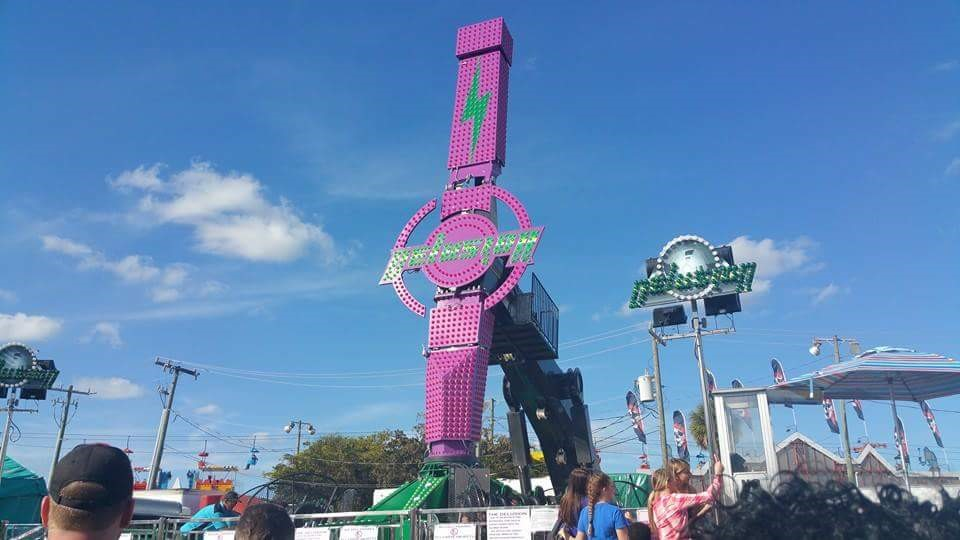
\includegraphics[width=125pt]{immagini/Pegasus.png}
					\label{Pegasus}
				\end{figure}		    
			\end{column}
		\end{columns}	    
	\end{frame}
%%%%%%%%%%%%%%%%%%%%%%%%%%%%%%%%%%%%%%%%%%%%%%%%%%%%%%%%%%%%%%%%%%%%%%%%%%%%%%%%	
	\begin{frame}{\small "WHAT WE WANT FROM THE SYSTEM?"}
		\textbf{GOALS}: Studying the system performing a \emph{kinematic} and \emph{dynamic} analysis and design an appropriate model to evaluate the system performance
		
		\medskip
		
		\begin{columns}
			\begin{column}{0.5\textwidth}
				\begin{figure}
					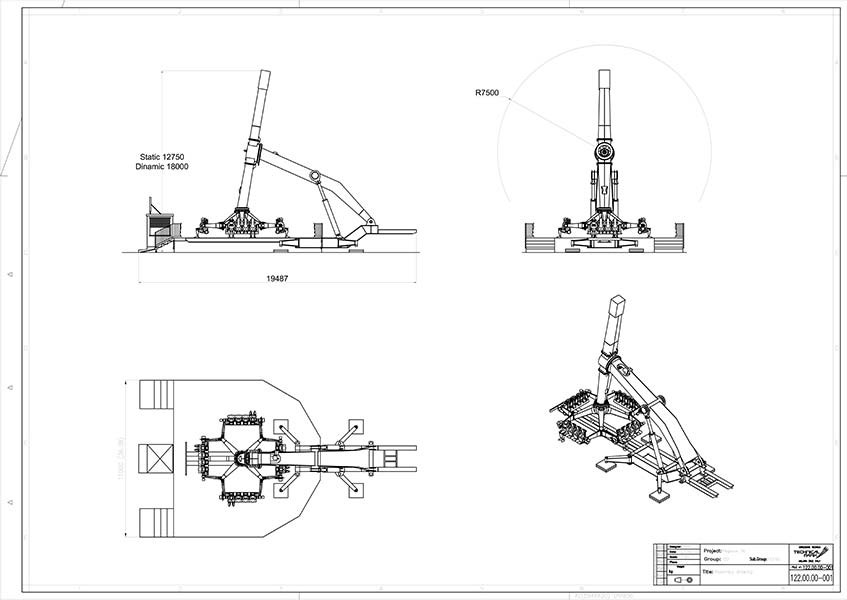
\includegraphics[width=150pt]{immagini/competitorsData.jpg}
					\label{disegno3D}
				\end{figure}	
			\end{column}
			\begin{column}{0.5\textwidth}
				\begin{figure}
					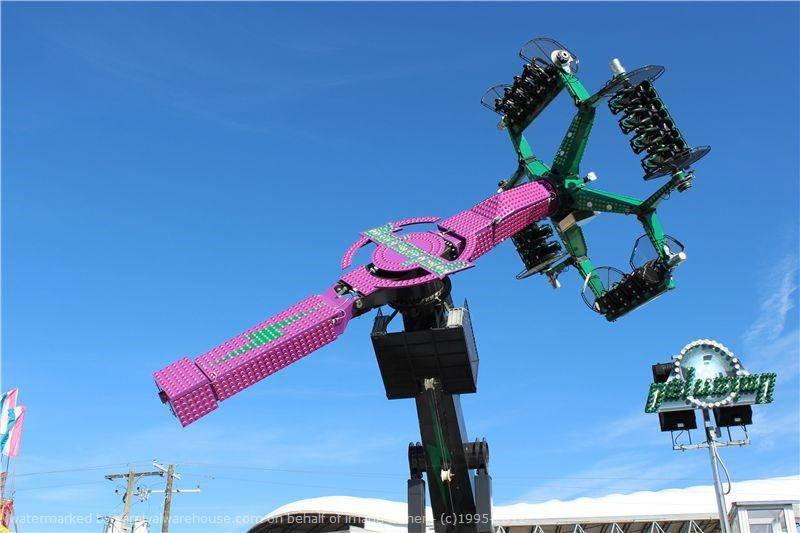
\includegraphics[width=150pt]{immagini/Pegasus2.jpg}
					\label{Pegasus2}
				\end{figure}
			\end{column}
		\end{columns}
	\end{frame}
%%%%%%%%%%%%%%%%%%%%%%%%%%%%%%%%%%%%%%%%%%%%%%%%%%%%%%%%%%%%%%%%%%%%%%%%%%%%%%%%	
	\begin{frame}{Quality Function Deployment (QFD)}
		\centering
		Following the \textbf{House of Quality} procedure to better develop engineering specifications and to satisfy the costumer needs
		
		\medskip
		
		\centering
		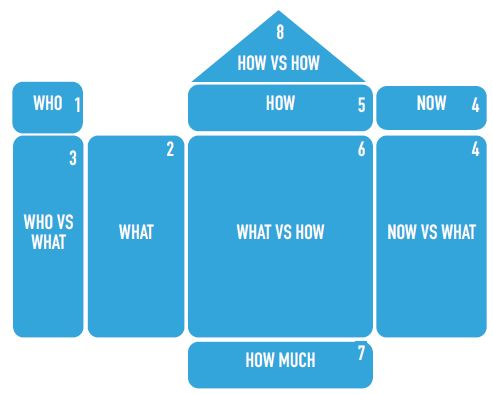
\includegraphics[width=200pt]{immagini/QFD.JPG}			
	\end{frame}
%%%%%%%%%%%%%%%%%%%%%%%%%%%%%%%%%%%%%%%%%%%%%%%%%%%%%%%%%%%%%%%%%%%%%%%%%%%%%%%%	
	\begin{frame}{System requirements}
		\large 
		
		We have extracted the following system requirements:
	
		\bigskip
		
		\begin{tasks}(2)				
			\task Enjoyable ride					
			\task Low energy consumption
			\task Space optimization									
			\task Passenger safety
			\task Suitable for passengers of different sizes
			\task Reduced motion sickness after the ride
			\task Durability of the structure
			\task Maximization of gains 	    
		\end{tasks}	
	\end{frame}	
%%%%%%%%%%%%%%%%%%%%%%%%%%%%%%%%%%%%%%%%%%%%%%%%%%%%%%%%%%%%%%%%%%%%%%%%%%%%%%%%
	\begin{frame}{Engineering specifications: KINEMATICS}
		\centering			
		
		\tiny	
		\begin{center}
			\begin{tabular}{p{2.8 cm} p{2.8 cm} p{2 cm} p{0.5 cm}}
				\toprule
				\textbf{System requirements}&\textbf{Engineering Specifications}  &\textbf{Target value} &\textbf{Unit} \\
				\toprule							
				& & $L=18\div19$ & \\ Space optimization & \hyperlink{1}{Workspace} & $W=16\div17$ & $m$ \\ & & $H=16\div18$ & \\
				\midrule				    
				Reduced motion sickness &\hyperlink{6}{Maximum angular velocity} & $9\div12$  & $rpm$  \\
				\midrule
				Maximization of gains & \hyperlink{7}{Theoretical hourly capacity} & $300 \div 380$ & $pph$   \\
				\midrule	      
				Passengers of different sizes & \hyperlink{8}{Passengers' height} & $<1.90$  & $m$  \\
				Passenger safety & & & \\
				\midrule
				Passenger safety &  & $Gx=-2\div+2\,g$&   \\
				Enjoyable ride& \hyperlink{3}{Maximum Acceleration}&$Gy=-2\div+2\,g$&$\frac{m}{s^{2}}$\\
				&&$Gz=-1.5\div+4\,g$&\\
				\midrule
				Low energy consumption& & & \\
				Durability of the structure & \hyperlink{5}{Time at max acceleration} & $<5$ &$s$\\
				Enjoyable ride & & &\\							
				\bottomrule
			\end{tabular}
		\end{center}	
	\end{frame}
%%%%%%%%%%%%%%%%%%%%%%%%%%%%%%%%%%%%%%%%%%%%%%%%%%%%%%%%%%%%%%%%%%%%%%%%%%%%%%%%	
	\begin{frame}{Engineering specifications: DYNAMICS}		
		\centering
		
		\tiny	
		\begin{center}
			\begin{tabular}{p{3 cm} p{3 cm} p{2 cm} p{0.5 cm}}
				\toprule
				\textbf{System requirements} &\textbf{Engineering specifications} &\textbf{Target value} &\textbf{Unit} \\
				\toprule		
				Low energy consumption & \hyperlink{2}{Weight of the structure} &$12000\div16000$ & $Kg$  \\ 				
				\midrule		
				Low energy consumption& \hyperlink{10}{Power} & $150\div200$ & $kW$ \\					
				\midrule				
				Passengers of different sizes  & & & \\
				Durability of the structure&\hyperlink{9}{Passengers' weight}  & $<130$ & $Kg$\\
				Low energy consumption&&&\\
				
				\bottomrule
			\end{tabular}
		\end{center}	
	\end{frame}
%%%%%%%%%%%%%%%%%%%%%%%%%%%%%%%%%%%%%%%%%%%%%%%%%%%%%%%%%%%%%%%%%%%%%%%%%%%%%%%%	
	\begin{frame}[fragile]{TARGET VALUES (part.1)}		
		
		\begin{itemize}
			\small
			
			\item \hypertarget{1}{\textbf{Workspace}}: it's one of the most important engineering specification of the system
			
			\medskip
			
			\begin{itemize}
				\scriptsize
				\item[$\rightarrow$] \url{https://www.technicalpark.com/amusement-rides/pegasus-16/}
				\item[$\rightarrow$] \url{https://www.technicalpark.com/amusement-rides/pegasus-30/}
				\item[$\rightarrow$] \url{https://www.zamperla.com/products/midi-discovery/}
			\end{itemize}
			
			\medskip
			
			\item \hypertarget{2}{\textbf{Weight of the structure}}: the weight range has been chosen from a competitor ride of similar dimensions:
			\textattachfile[color=0.0 0.72 0.92]{allegati/revolution32specsheet.pdf}{Revolution 32}
			
			\medskip
			
			\item \hypertarget{3}{\textbf{Maximum acceleration}}: the values has been chosen according to the study {\scriptsize \textattachfile[color=0.0 0.72 0.92]{allegati/hsl02-07.pdf}{Establishing criteria for safe g-force levels for passenger carrying amusement rides}} \\(pag.7)	
		\end{itemize}
	\end{frame}
%%%%%%%%%%%%%%%%%%%%%%%%%%%%%%%%%%%%%%%%%%%%%%%%%%%%%%%%%%%%%%%%%%%%%%%%%%%%%%%%	
	\begin{frame}[fragile]{TARGET VALUES (part.2)}
		\begin{itemize}
			\footnotesize				
			\item \hypertarget{5}{\textbf{Time at maximum Acceleration}}: appropriate values derived from the paper
			\textattachfile[color=0.0 0.72 0.92]{allegati/HighAccelerationandtheHumanBody.pdf}{High Acceleration and the Human Body} (pag.11)	
			
			\medskip
			
			\item \hypertarget{6}{\textbf{Maximum angular velocity}}: from \textattachfile[color=0.0 0.72 0.92]{allegati/AGEvidenceReport.pdf}{Artificial Gravity} (pag. 11) angular velocities can cause  motion sickness due to Coriolis forces and cross-coupled angular acceleration.		
			
			\medskip 
			
			\begin{itemize}
				\scriptsize
				\item[$\rightarrow$] \textattachfile[color=0.0 0.72 0.92]{allegati/AGEvidenceReport.pdf}{Artificial Gravity} (pag.42)
				\item[$\rightarrow$] \url{https://www.fabbrigroup.com/portfolio-item/inversion/#1506782277732-1147f336-5b75}
				\item[$\rightarrow$] \url{https://www.technicalpark.com/amusement-rides/pegasus-16/}
			\end{itemize}	
			
			\medskip
			
			\item \hypertarget{7}{\textbf{Theoretical hourly capacity}}: we obtained the ranges comparing different competitors:			
			\begin{itemize}
				\scriptsize
				\item[$\rightarrow$] \url{https://www.zamperla.com/products/midi-discovery/}
				\item[$\rightarrow$] \url{https://www.fabbrigroup.com/portfolio-item/inversion/#1506782277732-1147f336-5b75}
				\item[$\rightarrow$] \url{https://www.rideentertainment.com/extreme-rides/booster/}
			\end{itemize}	
		\end{itemize}
	\end{frame}
%%%%%%%%%%%%%%%%%%%%%%%%%%%%%%%%%%%%%%%%%%%%%%%%%%%%%%%%%%%%%%%%%%%%%%%%%%%%%%%%	
	\begin{frame}[fragile]{TARGET VALUES (part.3)}
		\begin{itemize}
			\small
			\item \hypertarget{10}{\textbf{Power}}: we selected the target from these competitors:			
			\begin{itemize}
				\scriptsize
				\item[$\rightarrow$] \url{https://www.rideentertainment.com/extreme-rides/booster/}
				\item[$\rightarrow$] \url{https://www.rideentertainment.com/extreme-rides/chaos-pendle/}
			\end{itemize}
			
			\medskip
			
			\item \hypertarget{8}{\textbf{Passengers' height}}:  we imposed the limit of man 95 percentile:	
			
			\medskip
			
			\begin{itemize}
				\scriptsize
				\item[$\rightarrow$] \url{https://www.rideentertainment.com/extreme-rides/chaos-pendle/}
				\item[$\rightarrow$] \url{https://www.rideentertainment.com/extreme-rides/booster/}
				\item[$\rightarrow$] \url{https://dqydj.com/height-percentile-calculator-for-men-and-women/}
			\end{itemize}
			
			\medskip
			
			\item \hypertarget{9}{\textbf{Passengers' weight}}: we imposed the limit of man 95 percentile:
			\begin{itemize}
				\scriptsize
				\item[$\rightarrow$] \url{https://dqydj.com/weight-percentile-calculator-men-women/}
				\item[$\rightarrow$] \textattachfile[color=0.0 0.72 0.92]{allegati/revolution32specsheet.pdf}{Revolution 32}
			\end{itemize}
			
		\end{itemize}
	\end{frame}
%%%%%%%%%%%%%%%%%%%%%%%%%%%%%%%%%%%%%%%%%%%%%%%%%%%%%%%%%%%%%%%%%%%%%%%%%%%%%%%%	
	\begin{frame}{PERFORMANCE INDICES}
		\begin{center}
			\begin{tabular}{lll}
				\toprule
				\textbf{Performance Index}  &\textbf{Target value} &\textbf{Unit} \\
				\toprule					
				& $L=18\div19$ & \\ 
				Workspace&$W=10\div13$ & $m$ \\
				& $H=16\div18$ & \\					
				Theoretical hourly capacity&$300 \div 380$ & $pph$  \\
				Acceleration profile& & $\frac{m}{s^{2}}$ \\				
				
				Power& $150\div200$ & $KW$ \\	
				\bottomrule
			\end{tabular}
		\end{center}	
	\end{frame}
%%%%%%%%%%%%%%%%%%%%%%%%%%%%%%%%%%%%%%%%%%%%%%%%%%%%%%%%%%%%%%%%%%%%%%%%%%%%%%%%	
	\begin{frame}{WEIGHTING MATRIX }
		\small
		
		\begin{columns}
			\begin{column}[t]{0.5\textwidth}
				\begin{block}{\small \centering Engineering specifications}
					
					\medskip
					
					\begin{tabular}{ll}
						\toprule
						\textbf{Specification} & \textbf{Rate} \\
						\toprule
						Maximum acceleration & 9 \\
						Workspace & 9 \\
						Maximum angular velocity & 8 \\
						Theoretical hourly capacity & 6 \\
						Time at max acceleration &  5\\
						Passengers' weight& 4\\			
						Passengers' height & 4 \\		
						Power & 3\\											
						Weight of the structure& 2 \\	
						\bottomrule
					\end{tabular}
				\end{block}	
			\end{column}
		\begin{column}[t]{0.5\textwidth}
			\begin{block}{\small \centering Performance indices}
				
				\medskip
				
				\begin{tabular}{ll}
					\toprule
					\textbf{Performance index}  & \textbf{Rate} \\
					\toprule					
					Workspace & 9 \\
					Acceleration Profile & 7 \\						
					Theoretical hourly capacity & 5 \\		
					Power & 2 \\		
					\bottomrule
				\end{tabular}
			\end{block}
			\end{column}
		\end{columns}
	\end{frame}
%%%%%%%%%%%%%%%%%%%%%%%%%%%%%%%%%%%%%%%%%%%%%%%%%%%%%%%%%%%%%%%%%%%%%%%%%%%%%%%%	
	\begin{frame}{KINEMATIC ANALYSIS}			
		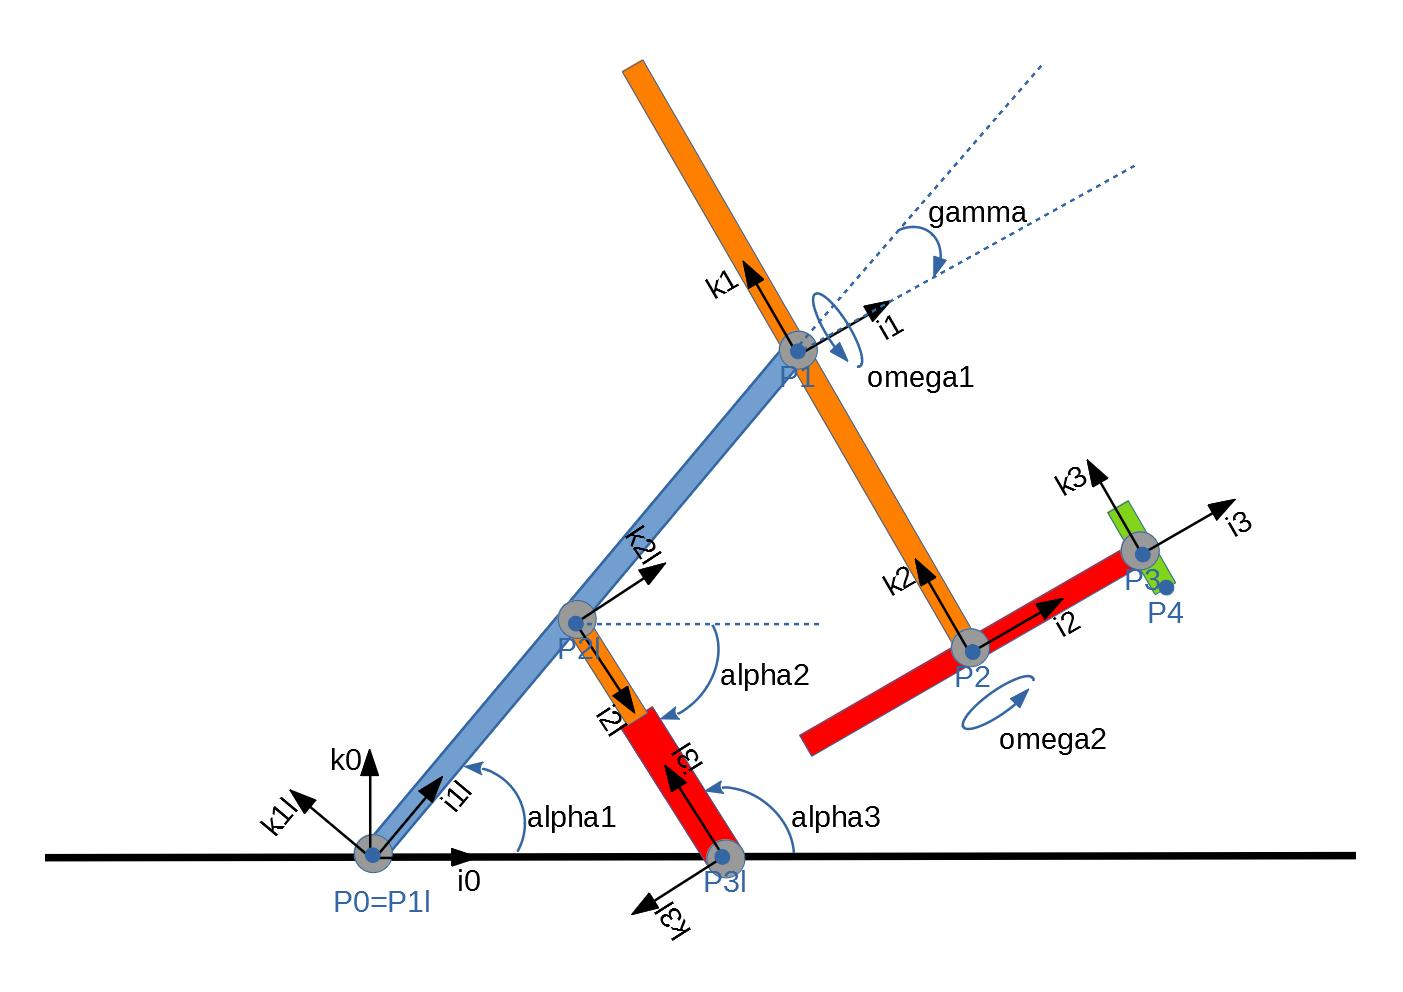
\includegraphics[width=300pt]{immagini/2D_pegasus.jpg}
	\end{frame}    
%%%%%%%%%%%%%%%%%%%%%%%%%%%%%%%%%%%%%%%%%%%%%%%%%%%%%%%%%%%%%%%%%%%%%%%%%%%%%%%%	
	\begin{frame}{Initial considerations}
		We did the following assumptions:
		
		\medskip 
		
		\begin{itemize}
			\item Rheonomous constraint for independent coordinates
			\begin{itemize}
				\item[$\rightarrow$] Constant angular velocities
			\end{itemize} 
			\item Lifting arm oriented along the X-axis
			\item Seats of passengers fixed to the Vehicle
			\item Lifting arm and Rotating arm analysed separately
			\item Rotating arm fixed with an angle of 30° with respect to the perpendicular to the Lifting arm
		\end{itemize}
	\end{frame}
%%%%%%%%%%%%%%%%%%%%%%%%%%%%%%%%%%%%%%%%%%%%%%%%%%%%%%%%%%%%%%%%%%%%%%%%%%%%%%%%	
	\begin{frame}{Recursive Approach}
		\small
		\begin{itemize}
			\item P0: origin on the ground 
			\item P1: Lifting - Rotating arm revolute joint
			\item P2: Rotating arm - center of the Vehicle revolute joint
			\item P3: Vehicle - last Seat revolute joint 
			\item P4: foot of the passenger
		\end{itemize}
		
		\medskip
		
		Since we consider the Lifting arm as fixed we have only two moving bodies: the Rotating arm (body1) and the Vehicle (body2)
		
		\smallskip
		
		Being an open chain mechanism, there are no constraint equations with this formulation  
	\end{frame}	    
%%%%%%%%%%%%%%%%%%%%%%%%%%%%%%%%%%%%%%%%%%%%%%%%%%%%%%%%%%%%%%%%%%%%%%%%%%%%%%%%	
	\begin{frame}{Global Approach}
		\small 
		Absolute coordinates and Euler angles sequence 
		\begin{itemize}
			\item[$\rightarrow$] $rot(Y,phi).rot(X,theta).rot(Z,psi)$
		\end{itemize}
		

		And as independent coordinates:		
		\begin{itemize}
			\item[$\rightarrow$] $psi2(t)$, $theta1(t)$
		\end{itemize} 
			
		\begin{columns}
			\begin{column}[t]{0.55\textwidth}	
				\begin{block}{\small \centering Constraint Equations}\scriptsize		
					\begin{itemize}
						\item I Revolute joint \\						
						(Lifting arm - Rotating arm)						
						\item II revolute joint \\
						(Rotating arm - Vehicle)						
						\item Time law of independent coordinates:
						
						{\tiny $PHI{\_}t := [theta1(t)-omega1{\cdot}t, psi2(t)-omega2{\cdot}t]$}
					\end{itemize}
				\end{block}	
			\end{column}
			\begin{column}[t]{0.45\textwidth}
				\begin{block}{\small \centering Newton-Raphson method}
					
					\bigskip 
					
					\footnotesize		
					 Numerical approach because of the high number of constraint equations
				\end{block}
			\end{column}	
		\end{columns}		
	\end{frame}	
%%%%%%%%%%%%%%%%%%%%%%%%%%%%%%%%%%%%%%%%%%%%%%%%%%%%%%%%%%%%%%%%%%%%%%%%%%%%%%%%
	\begin{frame}{Lifting Arm}
		\footnotesize 
		\begin{columns}
			\begin{column}{0.6\textwidth}
				\begin{block}{3-body system}
					\begin{itemize}
						\item[$\rightarrow$] Lifting arm \textcolor{blue}{(body1)}
						\item[$\rightarrow$] Piston \textcolor{orange}{(body2)}
						\item[$\rightarrow$] Chamber \textcolor{red}{(body3)}
					\end{itemize}
				\end{block}
				
				\medskip
				
				One degree of freedom: s(t) \\
				Initial condition of $alpha1=30$° \\
				Final condition $alpha1=50$° \\
				
				\medskip
				
				By means of Carnot's theorem we computed these lengths:
				
				\textcolor{blue}{$L1=14$ $m$},	
				\textcolor{orange}{$L2=3.62$ $m$}\\
				\textcolor{red}{$L3 = 3.62$ $m$}, $Lp = 7$ $m$\\
			\end{column}
			\begin{column}{0.4\textwidth}		
				\begin{figure}
					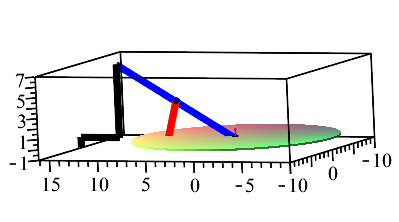
\includegraphics[width=125pt]{grafici/liftarm_initialpos.png}
				\end{figure}
				\begin{figure}
					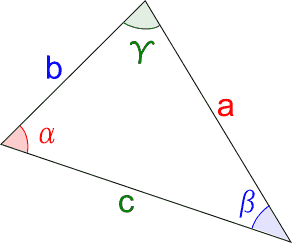
\includegraphics[width=75pt]{immagini/teorema_carnot.png}
				\end{figure}
			    \begin{equation*}
			     b^2=a^2+c^2-2ac\,cos(\beta)
			    \end{equation*}
			\end{column}	
		\end{columns}
	\end{frame}
%%%%%%%%%%%%%%%%%%%%%%%%%%%%%%%%%%%%%%%%%%%%%%%%%%%%%%%%%%%%%%%%%%%%%%%%%%%%%%%%	
	\begin{frame}{Animation of the mechanism}
		\small
		By connecting the Lifting arm with the main part of the system we got the final kinematic model of our amusement ride:	
			
		\begin{center}
			\animategraphics[loop,controls,width=0.5\textwidth]{10}{animations/p1e8k8iuatgaavho11pe1btie394-}{0}{29} \\
		\end{center}
	\end{frame}
%%%%%%%%%%%%%%%%%%%%%%%%%%%%%%%%%%%%%%%%%%%%%%%%%%%%%%%%%%%%%%%%%%%%%%%%%%%%%%%%	
	\begin{frame}{Position and Workspace Analysis}
		\begin{columns}
			\begin{column}{0.5\textwidth}
				\begin{block}{\centering Recursive}
					\centering
					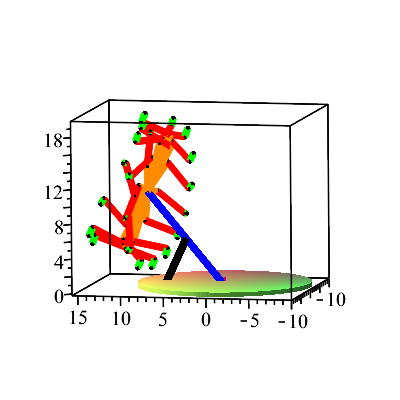
\includegraphics[width=100pt]{immagini/position_recursive.png}
					
					\medskip
					
					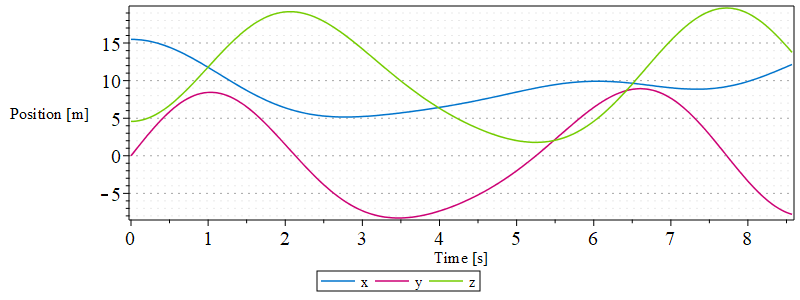
\includegraphics[width=150pt]{grafici/pos_pass_r.png}
				\end{block}
			\end{column}
			\begin{column}{0.5\textwidth}
				\begin{block}{\centering Global}
					\centering
					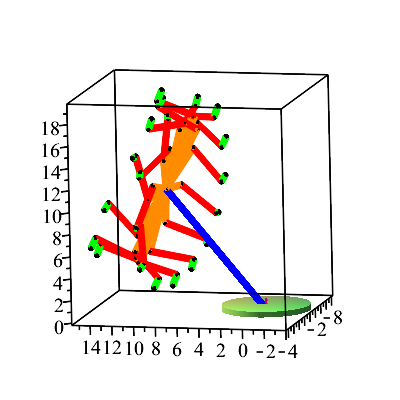
\includegraphics[width=100pt]{immagini/position_global.png}
					
					\medskip
					
					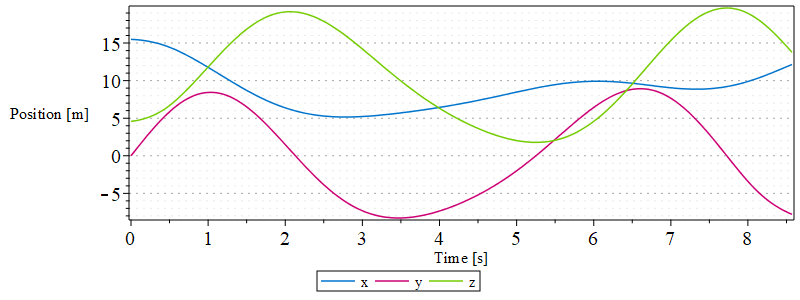
\includegraphics[width=150pt]{grafici/pos_pass_g.png}			
				\end{block}	
			\end{column}
		\end{columns}
	\end{frame}	
%%%%%%%%%%%%%%%%%%%%%%%%%%%%%%%%%%%%%%%%%%%%%%%%%%%%%%%%%%%%%%%%%%%%%%%%%%%%%%%%	
	\begin{frame}{Velocity and Acceleration Analysis}
		\begin{columns}
			\begin{column}{0.5\textwidth}
				\begin{block}{\centering Recursive}
				\end{block}
			\end{column}
			\begin{column}{0.5\textwidth}
				\begin{block}{\centering Global}
				\end{block}	
			\end{column}
		\end{columns}
		\centering Velocity perceived by the passenger
		\begin{columns}
			\begin{column}{0.5\textwidth}				
				\begin{figure}
					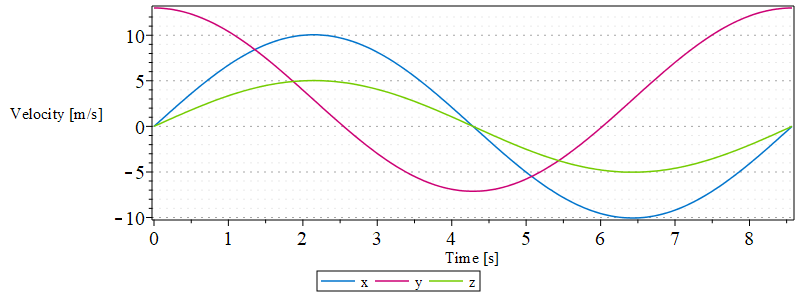
\includegraphics[width=150pt]{grafici/vel_pass_r.png}
				\end{figure}
			\end{column}
			\begin{column}{0.5\textwidth}
				\begin{figure}
					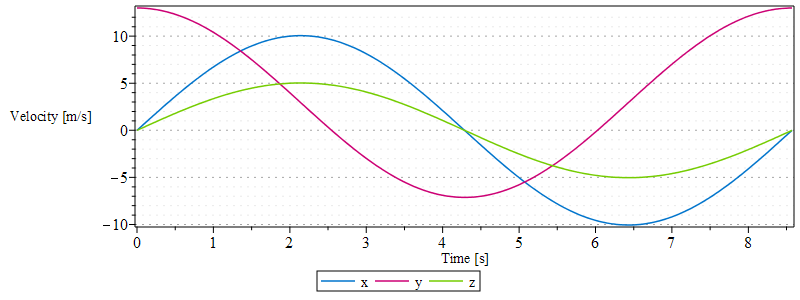
\includegraphics[width=150pt]{grafici/vel_pass_g.png}
				\end{figure}
			\end{column}
		\end{columns}	
		
		\medskip 
		
		\centering Acceleration perceived by the passenger
		\begin{columns}
			\begin{column}{0.5\textwidth}				
				\begin{figure}						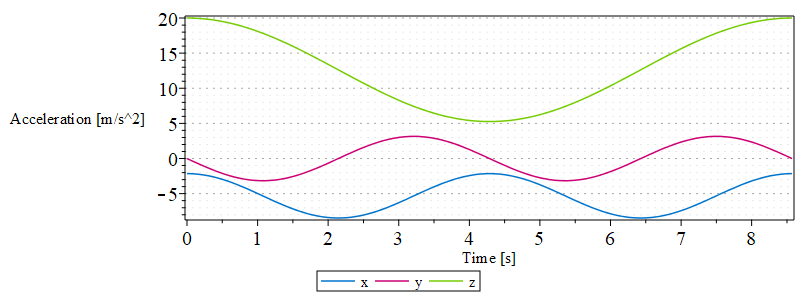
\includegraphics[width=150pt]{grafici/acc_pass_r.png}
				\end{figure}
			\end{column}
			\begin{column}{0.5\textwidth}
				\begin{figure}						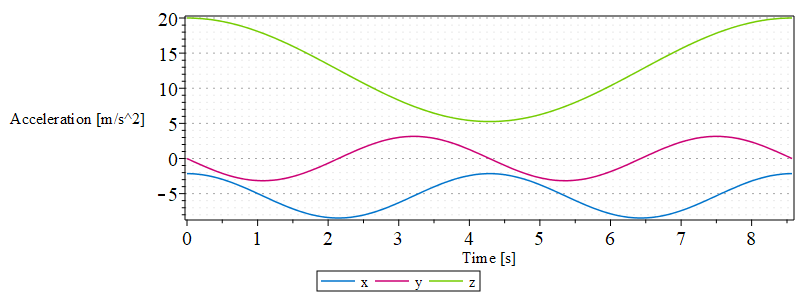
\includegraphics[width=150pt]{grafici/acc_pass_g.png}
				\end{figure}
			\end{column}
		\end{columns}
	\end{frame}
%%%%%%%%%%%%%%%%%%%%%%%%%%%%%%%%%%%%%%%%%%%%%%%%%%%%%%%%%%%%%%%%%%%%%%%%%%%%%%%%	
	\begin{frame}{Check of Engineering Specification (part.1)}
		\scriptsize

		\begin{itemize}
			\item \textbf{Workspace}: the results are obtained by observing the workspace configuration and the plots of position of the passenger
			
			\medskip
			
			\begin{center}
				\begin{tabular}{p{4 cm} p{2 cm} p{1.8 cm} p{0.5 cm} }
					\toprule
					\textbf{Engineering Specifications} &\textbf{Target value} &\textbf{Final value} & \textbf{Unit} \\
					\toprule							
					& $L=18\div19$ & $x\simeq15.5$ & \\ \centering Workspace & $W=16\div17$ & $y\simeq17$ & $m$ \\ & $H=16\div18$ & $z\simeq20$ & \\
					\midrule
				\end{tabular}
			\end{center}	
		\end{itemize}
		
		\medskip
		
		\begin{block}{\small \centering Parameters}
		\end{block}			
				\begin{tasks}(2)	
					\task[$\circ$] Length of the Lifting arm $L=14$ $m$ 
					\task[$\circ$] Half Rotating arm $L1=7$ $m$
					\task[$\circ$] Radius of the Vehicle $L2=4$ $m$  \\
					\task[$\circ$] Length of half Seat $L3=1$ $m$ 
					\task[$\circ$] Angle Lifting arm $alpha=50$° 
					\task[$\circ$] Angle Rotating arm - Lifting arm $gamma=30$°
				\end{tasks}	
	\end{frame}
%%%%%%%%%%%%%%%%%%%%%%%%%%%%%%%%%%%%%%%%%%%%%%%%%%%%%%%%%%%%%	
	\begin{frame}{Check of Engineering Specification (part.2)}
		\begin{itemize}
			\footnotesize	
			\item \textbf{Acceleration profile}:
			\begin{enumerate}
				\scriptsize
				\item along Z-axis: max acceleration at minimum height and no acceleration at maximum height 
				\item along Y-axis: zero
				\item along X-axis: constant acceleration $1\,g$
			\end{enumerate}			
		\end{itemize}	
		\begin{columns}
			\begin{column}{0.3\textwidth}		
				\centering Target profile
			\end{column}
			\begin{column}{0.7\textwidth}			
				\begin{figure}									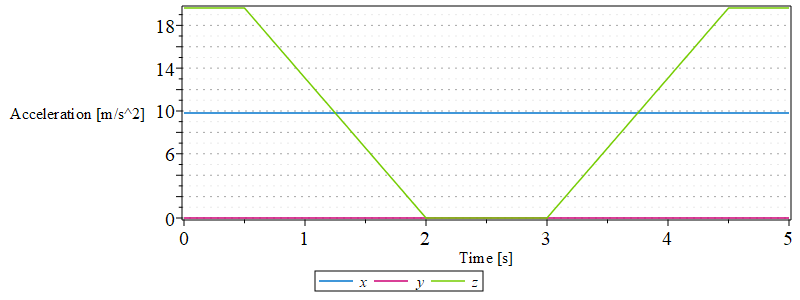
\includegraphics[width=175pt]{grafici/acc_profile.png}
				\end{figure}
			\end{column}
		\end{columns}
		\begin{columns}
			\begin{column}{0.3\textwidth}		
				\centering Difference between real profile and target profile
			\end{column}
			\begin{column}{0.7\textwidth}			
				\begin{figure}									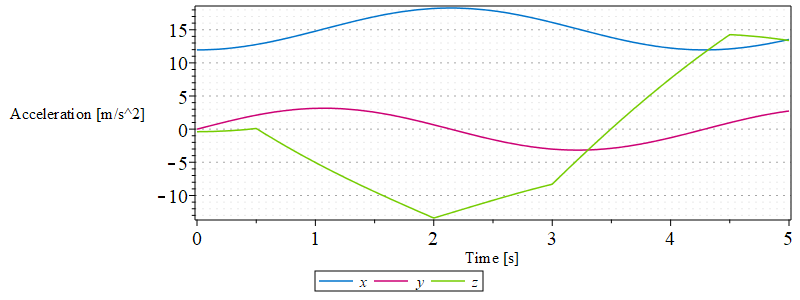
\includegraphics[width=175pt]{grafici/acc_distance.png}
				\end{figure}
			\end{column}
		\end{columns}		
	\end{frame}	
%%%%%%%%%%%%%%%%%%%%%%%%%%%%%%%%%%%%%%%%%%%%%%%%%%%%%%%%%%%%%	
	\begin{frame}{Check of Engineering Specification (part.3)}
		\small
		\begin{itemize}
			\item \textbf{Maximum angular velocity}: $2$ different angular velocities ($\omega_{1}$ for Rotating arm and $\omega_{2}$ for Crown)
			\begin{center}
				\begin{tabular}{p{4 cm} p{2 cm} p{1.5 cm} p{0.5 cm}}
					\textbf{} &\textbf{} &\textbf{} & \\						
					\centering $\omega_1$ & $9\div12$ & $10$ & $rpm$ \\ \centering $\omega_2$ & $9\div12$ & $7$ & $rpm$ \\
					\midrule
				\end{tabular}
			\end{center}
			
			\medskip
			
			\item \textbf{Theoretical hourly capacity}: 
			\begin{center}
				\begin{tabular}{p{4 cm} p{2 cm} p{1.5 cm} p{0.5 cm}}
					\textbf{} &\textbf{} &\textbf{} & \\						
					\centering Theoretical hourly capacity & $300 \div 380$ & $320$ & $pph$ \\ \centering Ride time & & $3$ & $min$ \\
					\midrule
				\end{tabular}
			\end{center}		
		\end{itemize}
	\end{frame}
%%%%%%%%%%%%%%%%%%%%%%%%%%%%%%%%%%%%%%%%%%%%%%%%%%%%%%%%%%%%%	
	\begin{frame}{Check of Engineering Specification (part.4)}
		\begin{itemize}
			\scriptsize
			\item \textbf{Maximum acceleration}: the results are obtained from the plots of the accelerations perceived by passengers
			\begin{center}
				\begin{tabular}{p{4 cm} p{2 cm} p{1.8 cm} p{0.5 cm}}
					\textbf{} &\textbf{} &\textbf{} & \\						
					\centering $Gx$ & $-2\div+2\,g$ & $\simeq-8.5\div-2.1$ & \\ 
					\centering $Gy$ & $-2\div+2\,g$ & $\simeq-3.2\div+3.2$ & $\frac{m}{s^{2}}$ \\
					\centering $Gz$ & $-1.5\div+4\,g$ & $\simeq5\div20$ & \\
					\midrule
				\end{tabular}
			\end{center}
			
			\medskip 
			
			\item \textbf{Time at max acceleration}: in the worst case it is around $1 \, sec$ 
			\begin{center}
				\begin{tabular}{p{4 cm} p{2 cm} p{1.8 cm} p{0.5 cm}}
					\textbf{} &\textbf{} &\textbf{} & \\							
					\centering Time at max acceleration & $<5$ & $1$ & $s$ \\ 
					\midrule
				\end{tabular}
			\end{center}
		\end{itemize}
	
	\medskip
	
	\centering
	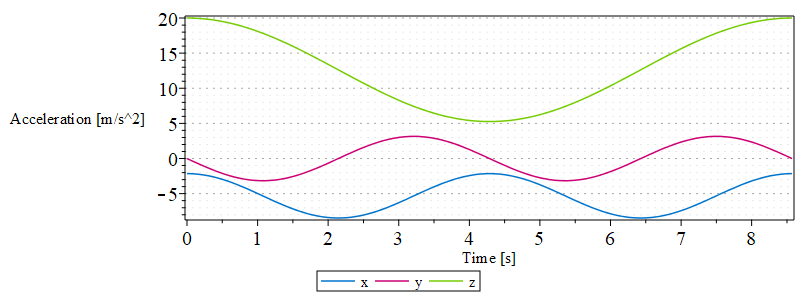
\includegraphics[width=200pt]{grafici/acc_pass_r.png}
	\end{frame}
%%%%%%%%%%%%%%%%%%%%%%%%%%%%%%%%%%%%%%%%%%%%%%%%%%%%%%%%%%%%%	
	\begin{frame}{DYNAMICS ANALYSIS}{INITIAL CONSIDERATIONS}
		We did the following assumptions:
		
		\medskip 
		
		\begin{itemize}
			\item Recursive formulation with Lagrange approach
			\item Iron density and rectangular prism consideration for masses
			\begin{itemize}
				\item[$\rightarrow$] $S=0.04 \, m^2$
				\item[$\rightarrow$] $\rho=7870 \, \frac{kg}{m^3}$
			\end{itemize}
			\item Rods approximation for bodies with mass distributed along an axis
			\item Seats not fixed to the Vehicle
			\item Start with a vertical seat 
			\item Constant angular velocities for independents coordinates
			\item Lifting arm and Rotating arm analyzed separately
		\end{itemize}
	\end{frame}
%%%%%%%%%%%%%%%%%%%%%%%%%%%%%%%%%%%%%%%%%%%%%%%%%%%%%%%%%%%%%
	\begin{frame}{Lagrange Approach}
		\scriptsize	
		\begin{columns}
			\begin{column}[T]{0.5\textwidth}
				\begin{block}{\small Definition of the bodies}	
					\begin{itemize}
						\item Rotating arm 					
						\item Vehicle					
						\item Seat
					\end{itemize}
				\end{block}
				\begin{block}{\small Actuation forces}\scriptsize		
					\begin{itemize}
						\item C1: motor torque which produce a rotation of the Rotating arm 				
						\item C2: motor torque which produce a rotation of the vehicle					
					\end{itemize}
				\end{block}
				\begin{block}{\small Parameters}\scriptsize		
					\begin{itemize}
						\item m: mass of the body			
						\item Ixx,Iyy,Izz,Ixy,Ixz,Iyz: moments of inertia respect each axis
						\item $lambda1,lambda2$: lagrange multipliers
					\end{itemize}
				\end{block}
			\end{column}
			\begin{column}[T]{0.5\textwidth}
		    	\begin{block}{\small Two different approaches}
			    	\begin{itemize}
			    		\item[$\rightarrow$] Constraint imposed by Lagrange multipliers considering zero external forces. Comparison with different solving approaches:
			    		\begin{itemize}
			    			\scriptsize
			    			\item[$\ast$] Maple solver
			    			\item[$\ast$] Matlab: Index reduction
			    			\item[$\ast$] Matlab: Projection method 
			    			\item[$\ast$] Matlab: Baumgarte stabilization
			    		\end{itemize}
					   \item[$\rightarrow$] Inverse dynamics substituting the constraint directly in the equations
			    	\end{itemize}
		  		\end{block}
			\end{column}
		\end{columns} 	
	\end{frame}	
%%%%%%%%%%%%%%%%%%%%%%%%%%%%%%%%%%%%%%%%%%%%%%%%%%%%%%%%%%%%%%%%%%%%%%%%%%%%%%%%%%%%%%%%%%%%%%%	
	\begin{frame}{Maple solver: DAE}		
		\begin{columns}
			\begin{column}{0.5\textwidth}
				\begin{block}{\small \centering $\theta_1$ and $\dot{\theta_1}$}
					\begin{figure}
						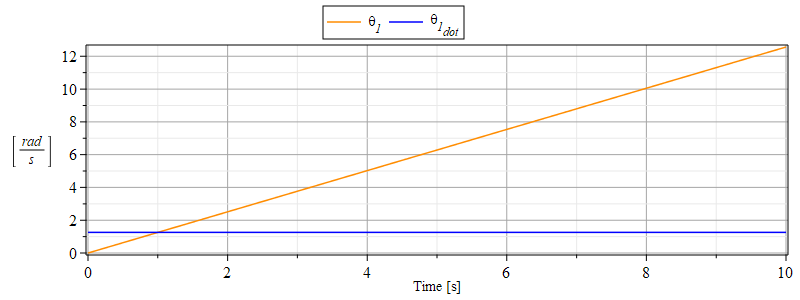
\includegraphics[width=150pt]{grafici/theta1_pos_vel.png}
					\end{figure}
				\end{block}
				\begin{block}{\small \centering $\theta_3$ and $\dot{\theta_3}$}
					\begin{figure}
						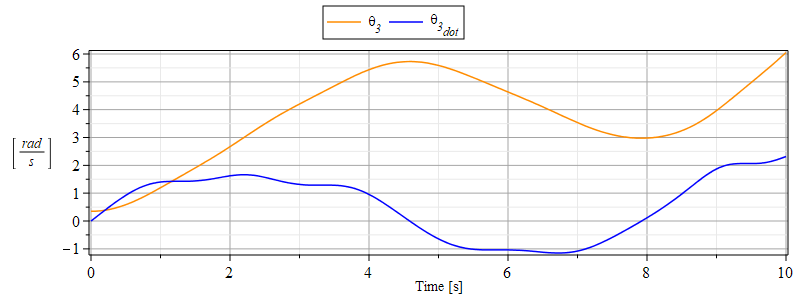
\includegraphics[width=150pt]{grafici/theta3_pos_vel.png}
					\end{figure}
				\end{block}
			\end{column}
			\begin{column}{0.5\textwidth}
				\begin{block}{\small \centering $\theta_2$ and $\dot{\theta_2}$}
					\begin{figure}
						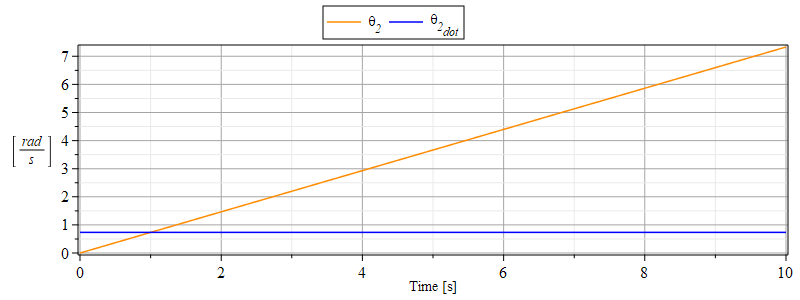
\includegraphics[width=150pt]{grafici/theta2_pos_vel.png}
					\end{figure}
				\end{block}
				\begin{block}{\centering \small $\lambda_1$ and $\lambda_2$}
					\begin{figure}
						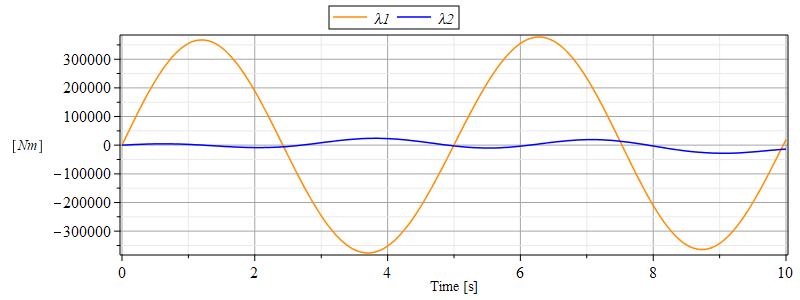
\includegraphics[width=150pt]{grafici/lambda1and2.png}
					\end{figure}
				\end{block}
			\end{column}
		\end{columns}
	\end{frame}
%%%%%%%%%%%%%%%%%%%%%%%%%%%%%%%%%%%%%%%%%%%%%%%%%%%%%%%%%%%%%%%%%%%%%%%%%%%%%%%%%%%%%%%%%%%%%%%	
	\begin{frame}{Maple solver: inverse Dynamics}
		\begin{columns}
			\begin{column}{0.5\textwidth}
				\begin{block}{\small \centering $\theta_3$ and $\dot{\theta_3}$}
					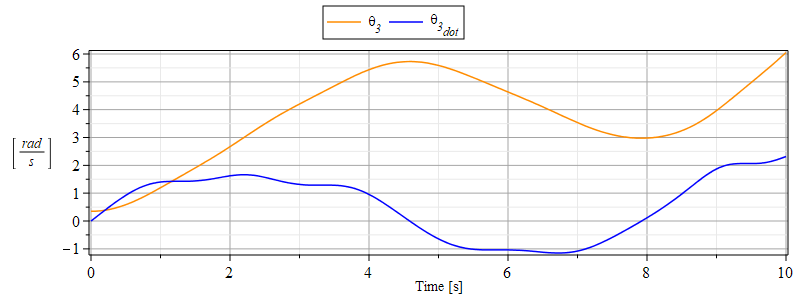
\includegraphics[width=150pt]{grafici/inverseDynamicsTheta.png}
				\end{block}
			\end{column}
		    \begin{column}{0.5\textwidth}
		     	\begin{block}{\small \centering $C_1$ and $C_2$}
		    		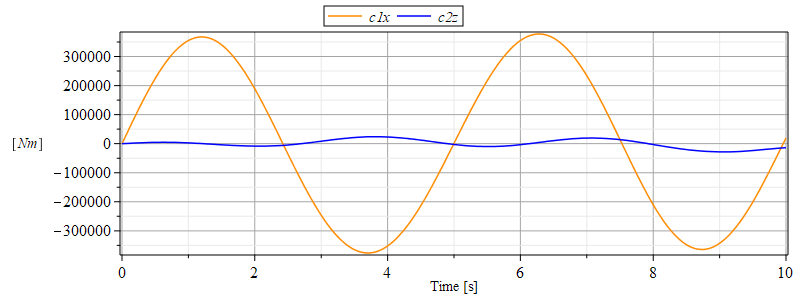
\includegraphics[width=150pt]{grafici/inverseDynamicsC.png}
		    	\end{block}
		    \end{column}
		\end{columns}
	
		\bigskip
		
		\begin{itemize}
			\item The values for $theta3$ are very similar to the  one obtained from the DAE
			\item We have the confirmation that the Lagrange multipliers coincide with the torques
		\end{itemize}    
	\end{frame}
%%%%%%%%%%%%%%%%%%%%%%%%%%%%%%%%%%%%%%%%%%%%%%%%%%%%%%%%%%%%%%%%%%%%%%%%%%%%%%%%%%%%%%%%%%%%%%%
	\begin{frame}{Analysis with MATLAB}
		\small
		By means of professor Bertolazzi's libraries we performed the following operations:
		\begin{itemize}
			\item Index reduction from index 3 to index 1 
			\item Transcription of the mechanism model from Maple to Matlab
			\begin{itemize}
				\item[$\ast$]  mass matrix 
				\item[$\ast$]  hidden constraint
				\item[$\ast$]  generalized forces
				\item[$\ast$]  jacobian of the RHS (implicit methods)
			\end{itemize}
		    \item Solving of the obtained DAE with:
		    \begin{itemize}
		    	\item[$\ast$]  implicit method (Radau) 
		    	\item[$\ast$]  projection method (Radau\_P)
		    	\item[$\ast$]  Baumgarte stabilization (Heun)
		    \end{itemize}
		\end{itemize}
	\end{frame}

%%%%%%%%%%%%%%%%%%%%%%%%%%%%%%%%%%%%%%%%%%%%%%%%%%%%%%%%%%%%%%%%%%%%%%%
	\begin{frame}{RESULTS implicit method}		
		\begin{columns}
			\begin{column}{0.33\textwidth}
			  	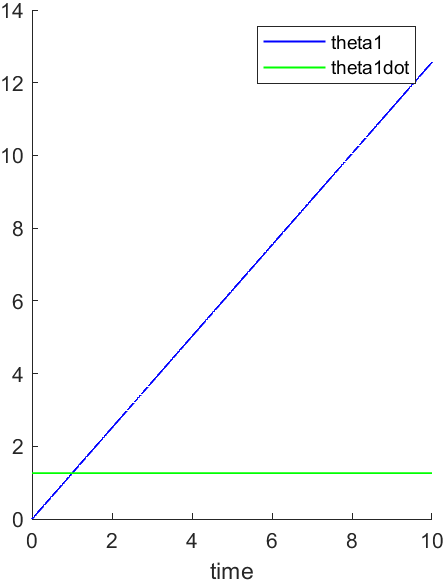
\includegraphics[width=100pt]{grafici/matlabNorm1.png}
			\end{column}
		    \begin{column}{0.33\textwidth}
		    	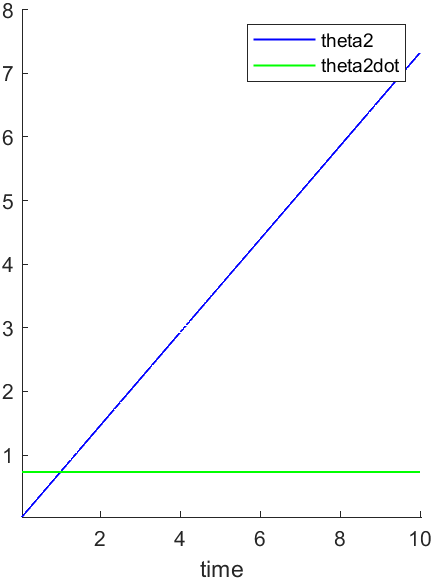
\includegraphics[width=100pt]{grafici/matlabNorm2.png}
		    \end{column}
		    \begin{column}{0.33\textwidth}
				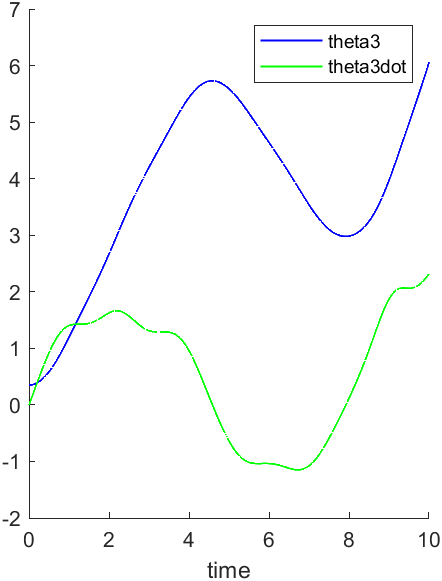
\includegraphics[width=100pt]{grafici/matlabNorm3.png}
		    \end{column}
		\end{columns}
	\end{frame}		
%%%%%%%%%%%%%%%%%%%%%%%%%%%%%%%%%%%%%%%%%%%%%%%%%%%%%%%%%%%%%%%%%%%%%%%%%%%%%%%%%%%%%%%%%%%%%%%	
	\begin{frame}{RESULTS Projection method}
		\begin{columns}
			\begin{column}{0.33\textwidth}
				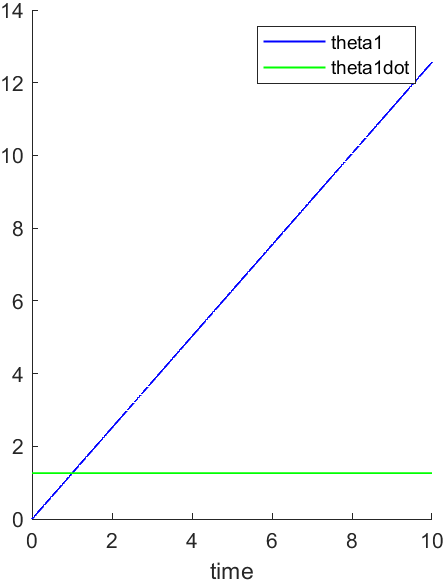
\includegraphics[width=100pt]{grafici/matlabProj1.png}
			\end{column}
			\begin{column}{0.33\textwidth}
				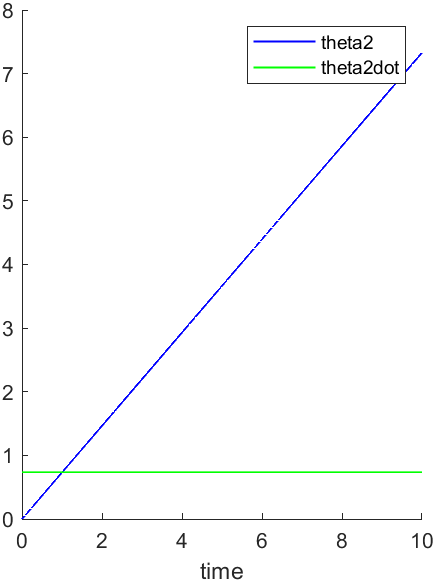
\includegraphics[width=100pt]{grafici/matlabProj2.png}
			\end{column}
			\begin{column}{0.33\textwidth}
				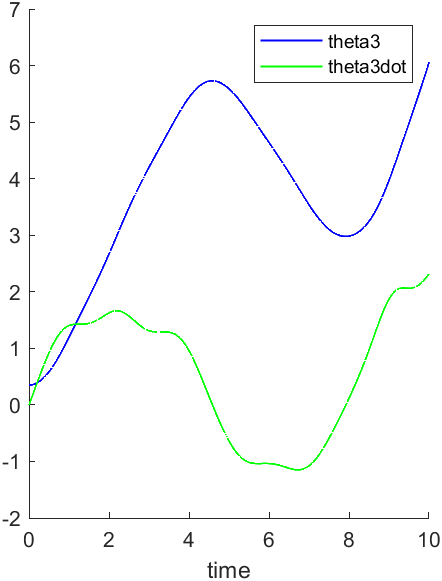
\includegraphics[width=100pt]{grafici/matlabProj3.png}
			\end{column}
		\end{columns}
	\end{frame}	
%%%%%%%%%%%%%%%%%%%%%%%%%%%%%%%%%%%%%%%%%%%%%%%%%%%%%%%%%%%%%%%%%%%%%%%%%%%%%%%%%%%%%%%%%%%%%%%	
	\begin{frame}{RESULTS Baumgarte stabilization}
		\begin{columns}
			\begin{column}{0.33\textwidth}
				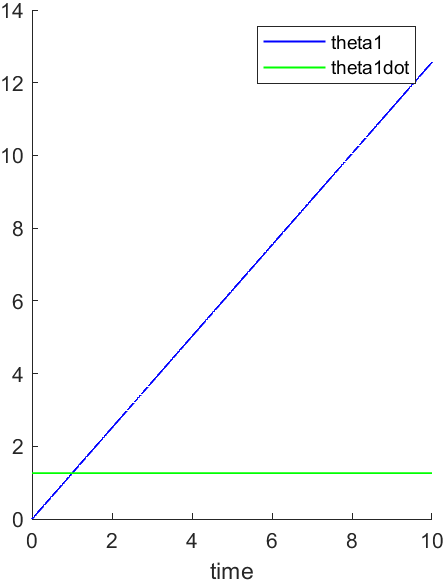
\includegraphics[width=100pt]{grafici/matlabBaung1.png}
			\end{column}
			\begin{column}{0.33\textwidth}
				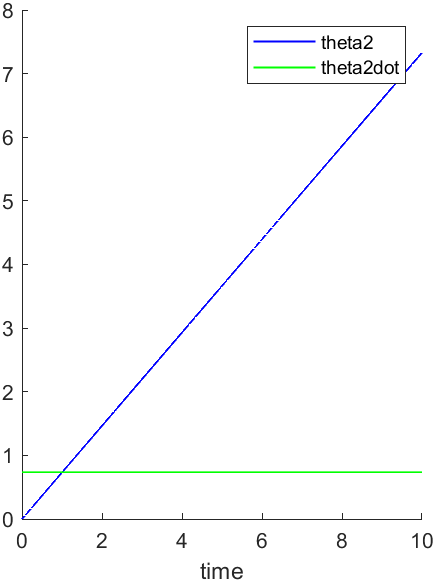
\includegraphics[width=100pt]{grafici/matlabBaung2.png}
			\end{column}
			\begin{column}{0.33\textwidth}
				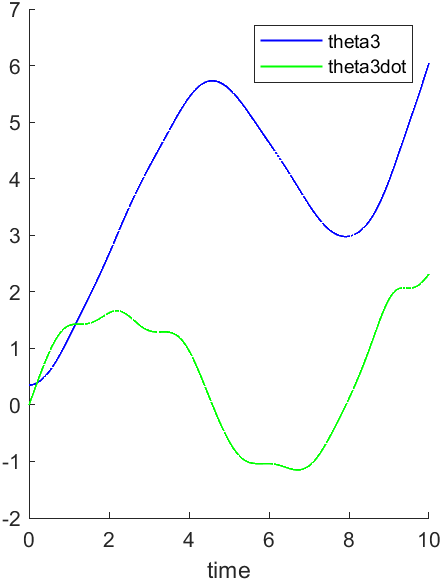
\includegraphics[width=100pt]{grafici/matlabBaung3.png}
			\end{column}
		\end{columns}
	\end{frame}
%%%%%%%%%%%%%%%%%%%%%%%%%%%%%%%%%%%%%%%%%%%%%%%%%%%%%%%%%%%%%%%%%%%%%%%%%%%%%%%%%%%%%%%%%%%%%%%	
	\begin{frame}{Lifting Arm}
		\footnotesize 	
		\centering
		We have the following differences:
		
		\smallskip
		
		\begin{tasks}(2)
			\task closed-loop mechanism\\ (3 constraint equations)
			\task constant force of the prismatic joint $F_0=\,50000\, N$ 
			\task no rheonomous constraint
			\task independent coordinate $s(t)$
		\end{tasks}
	\medskip
	    \begin{columns}
	    	\begin{column}{0.5\textwidth}
	    		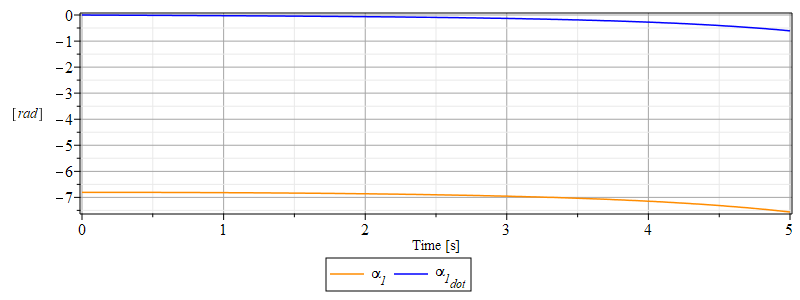
\includegraphics[width=150pt]{grafici/alpha1.png}
	    		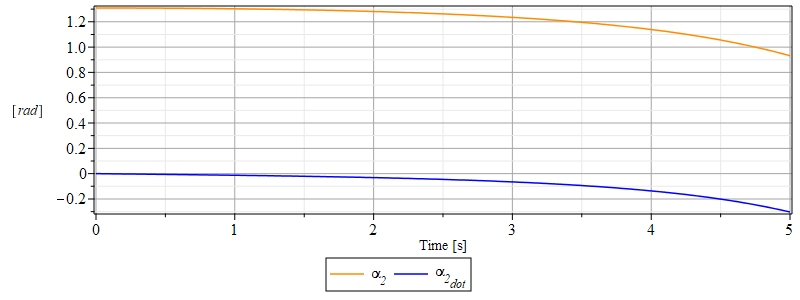
\includegraphics[width=150pt]{grafici/alpha2.png}
	    	\end{column}
	    	\begin{column}{0.5\textwidth}
	    		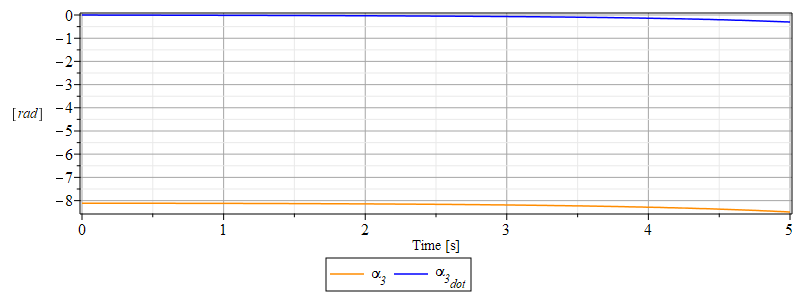
\includegraphics[width=150pt]{grafici/alpha3.png}
	    		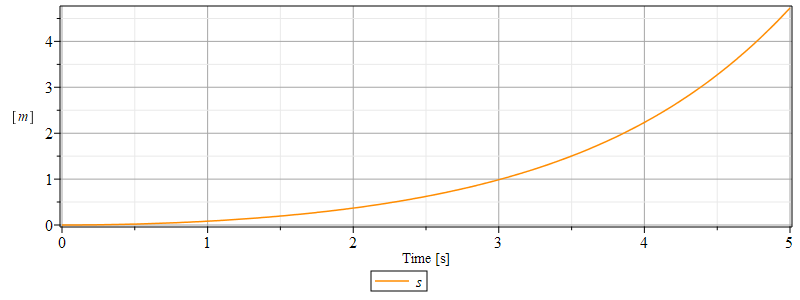
\includegraphics[width=150pt]{grafici/s.png}
	    	\end{column}
	    \end{columns}
				
	\end{frame}	
%%%%%%%%%%%%%%%%%%%%%%%%%%%%%%%%%%%%%%%%%%%%%%%%%%%%%%%%%%%%%%%%%%%%%%%%%%%%%%%%%%%%%%%%%%%%%%%	
	\begin{frame}{Check of Engineering Specification}
		\footnotesize		
		\begin{itemize}
			\item \textbf{Weight of the structure}: summing all masses we got: \\
			\begin{center}
				$M_{tot}=16762.13kg$
			\end{center}	
			
			\smallskip
			
			\item \textbf{Power}: sum of the power of the torque C1 and C2
			
			\medskip
			
			We can't compare it directly to the chosen index performance for the following reasons :
		\end{itemize}		
		\begin{columns}
			\begin{column}{0.5\textwidth}
				\begin{figure}
					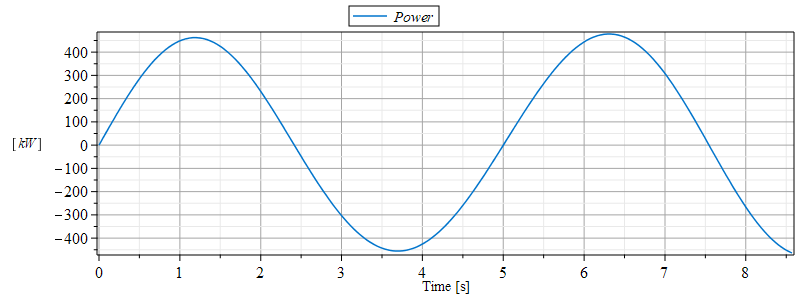
\includegraphics[width=150pt]{grafici/power.png}
				\end{figure}
			\end{column}
	     	\begin{column}{0.5\textwidth}			 
			 \begin{itemize}
			 	\item this power is purely mechanical
			 	\item oscillating power and average(RMS) has to be computed
			 	\item negative power during deceleration has not to be considered
			 \end{itemize}
	    	\end{column}
		\end{columns}
	
		\medskip
		
		\begin{center}
			\begin{tabular}{p{4 cm} p{2 cm} p{1.8 cm} p{0.5 cm} }
				\toprule
				\textbf{Engineering Specifications} &\textbf{Target value} &\textbf{Final value} & \textbf{Unit} \\
				\toprule							
				\centering Weight of the structure & $12000\div16000$ & $\simeq16700$ & $kg$ \\
				\midrule
				\centering Power & $150\div200$ & $-450\div450$ & $kW$ \\
				\bottomrule
			\end{tabular}
		\end{center}
	\end{frame}
	\begin{frame}{}
		\centering \textcolor{blue}{{\Huge  THANKS FOR THE \\
			\vspace{1cm} 
			ATTENTION }}
	\end{frame}
%%%%%%%%%%%%%%%%%%%%%%%%%%%%%%%%%%%%%%%%%%%%%%%%%%%%%%%%%%%%%%%%%%%%%%%%%%%%%%%%%%%%%%%%%%%%%%%	
\end{document}